In this section, we show the results obtained through the different numerical experiments,  conducted across different parameter constellations for the rBergomi model. Details about these examples are presented in Table \ref{table:Reference solution, using MC with $500$ time steps, of Call option price under rBergomi model, for different parameter constellation.}. The first set is the one that is closest to the empirical findings \cite{bennedsen2016decoupling,gatheral2018volatility}, which suggest that $H \approx 0.1$. The choice of parameter values of $\nu= 1.9$ and $\rho=-0.9$ is justified by \cite{bayer2016pricing}, where it is shown that these values are remarkably consistent with the SPX market on $4$th February $2010$. For the remaining three sets in Table \ref{table:Reference solution, using MC with $500$ time steps, of Call option price under rBergomi model, for different parameter constellation.}, we wanted to test the potential of our method for a very rough case, that is $H=0.02$, for three different  scenarios  of moneyness, $S_0/K$. In fact, hierarchical variance reduction methods, such as Multi-level Monte Carlo (MLMC), are inefficient in this context because of the poor behavior of the strong error, that is of the order of $H$ \cite{neuenkirch2016order}. We emphasize that we checked the robustness of our method for other parameter sets, but for illustrative purposes, we only show results for the parameters sets presented in Table \ref{table:Reference solution, using MC with $500$ time steps, of Call option price under rBergomi model, for different parameter constellation.}. For all our numerical experiments, we consider   a number of time steps $N \in \{2,4,8,16\}$, and  all reported errors are relative errors, normalized by the reference solutions provided in Table \ref{table:Reference solution, using MC with $500$ time steps, of Call option price under rBergomi model, for different parameter constellation.}.

\FloatBarrier
\begin{table}[!h]
	\centering
	\begin{small}
	\begin{tabular}{l*{2}{c}r}
	\toprule[1.5pt]
		Parameters            & Reference solution    \\
		\hline

			Set $1$:	$H=0.07, K=1,S_0=1, T=1, \rho=-0.9, \eta=1.9,\xi_0=0.235^2$   & $\underset{(5.6e-05)}{0.0791}$  \\	

				Set $2$:	$H=0.02, K=1, S_0=1, T=1,\rho=-0.7, \eta=0.4,\xi_0=0.1$   & $\underset{(9.0e-05)}{0.1246}$  \\
					Set $3$:	$H=0.02, K=0.8,S_0=1,T=1, \rho=-0.7, \eta=0.4,\xi_0=0.1$   & $\underset{(5.4e-05)}{0.2412}$  \\
						Set $4$:	$H=0.02, K=1.2,S_0=1,T=1, \rho=-0.7, \eta=0.4,\xi_0=0.1$   & $\underset{(8.0e-05)}{0.0570}$  \\
	\bottomrule[1.25pt]
	\end{tabular}
\end{small}
	\caption{Reference solution, which is the  approximation of the call option price under the rBergomi model, defined in \eqref{BS_formula_rbergomi},  using MC with $500$ time steps and number of samples, $M=8 \times 10^6$, for different parameter constellations.  The numbers between parentheses correspond to the statistical errors estimates.}
	\label{table:Reference solution, using MC with $500$ time steps, of Call option price under rBergomi model, for different parameter constellation.}
\end{table}
\FloatBarrier

\subsection{Weak error} \label{sec:Weak error plots_no_change}
We start our numerical experiments \red{by} accurately  estimating the weak error (bias), discussed in Section \ref{sec:Weak error analysis}, for the different parameter sets  in Table \ref{table:Reference solution, using MC with $500$ time steps, of Call option price under rBergomi model, for different parameter constellation.}, with and without Richardson extrapolation.   For illustrative purposes, we only show the weak errors related to set $1$ in Table \ref{table:Reference solution, using MC with $500$ time steps, of Call option price under rBergomi model, for different parameter constellation.} (see Figure \ref{fig:Weak_rate_set1_set_2_without_rich}). We note that we observed similar behavior for the other parameter sets, with slightly worse rates for some cases. We emphasize that the reported weak rates correspond to the pre-asymptotic regime that we are interested in. We are not interested in estimating the rates specifically but rather obtaining  a sufficiently precise estimate of the weak error (bias), $\mathcal{E}_B(N)$, for different  numbers of time steps $N$.  For a fixed discretization, the corresponding estimated biased solution will be set as a reference solution to the  ASGQ method  in order to estimate the quadrature error $\mathcal{E}_Q(\text{TOL}_{\text{ASGQ}},N)$.	
\FloatBarrier
\begin{figure}[h!]
	\centering
	\begin{subfigure}{.4\textwidth}
		\centering
		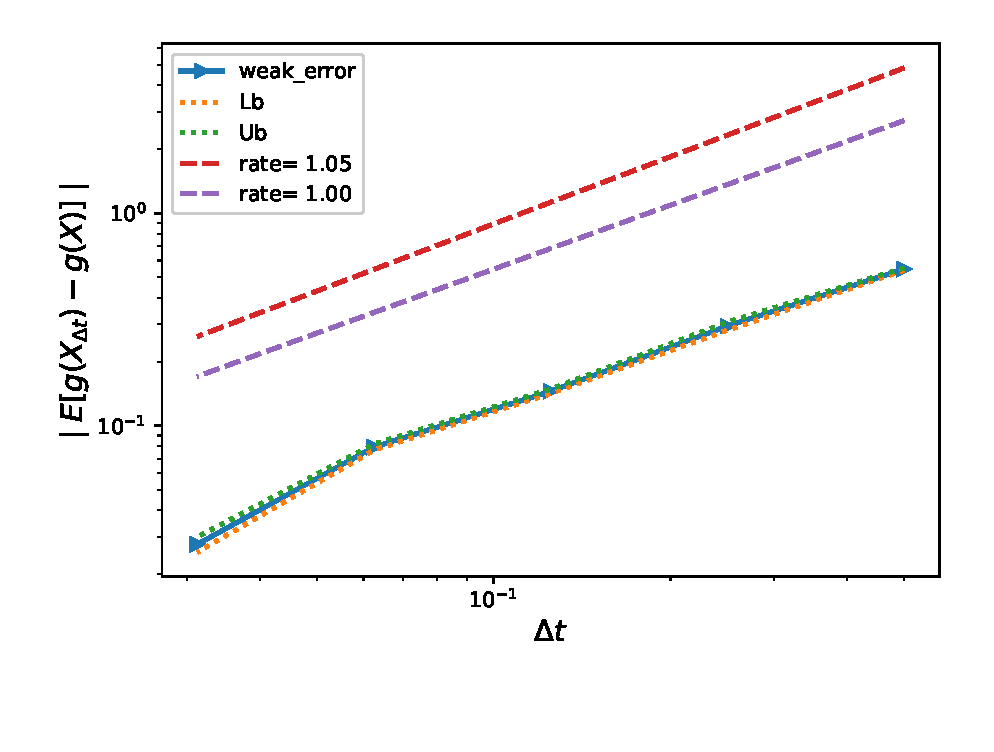
\includegraphics[width=1\linewidth]{./figures/rBergomi_weak_error_rates/without_richardson/H_007/weak_convergence_order_Bergomi_H_007_K_1_M_10_6_CI_relative}
		\caption{}
		\label{fig:sub3}
	\end{subfigure}%
	\begin{subfigure}{.4\textwidth}
		\centering
		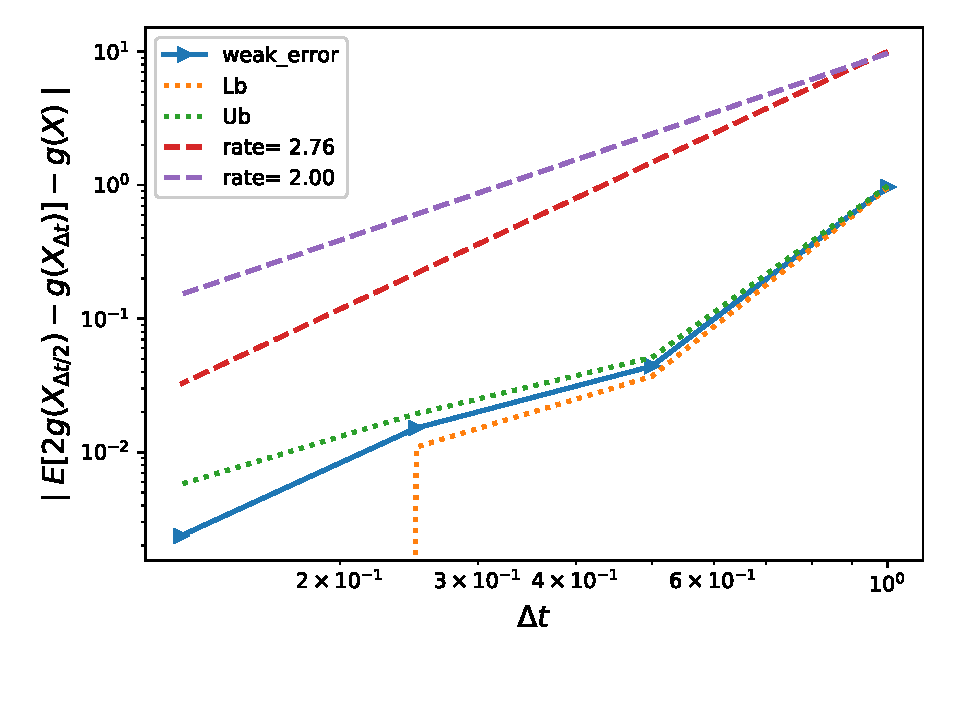
\includegraphics[width=1\linewidth]{./figures/rBergomi_weak_error_rates/with_richardson/H_007/weak_convergence_order_Bergomi_H_007_K_1_richardson_relative_M_10_6}
		\caption{}
		\label{fig:sub4}
	\end{subfigure}
	
	\caption{The  convergence of the weak error $\mathcal{E}_B(N)$, defined in \eqref{eq: Weak_error_hyb_chol}, using MC, for set $1$ parameter in Table \ref{table:Reference solution, using MC with $500$ time steps, of Call option price under rBergomi model, for different parameter constellation.}. We refer to $C_{\text{RB}}$ as $\expt{g(X)}$, and to $C_{\text{RB}}^{N}$ as  $\expt{g(X_{\Delta t})}$. The upper and lower bounds are $95\%$ confidence intervals. a) without Richardson extrapolation.  b) with Richardson extrapolation (level $1$).}
	\label{fig:Weak_rate_set1_set_2_without_rich}
\end{figure}
\FloatBarrier


%
%\begin{figure}[!htb]
%	\centering
%	\begin{subfigure}{.35\textwidth}
%		\centering
%		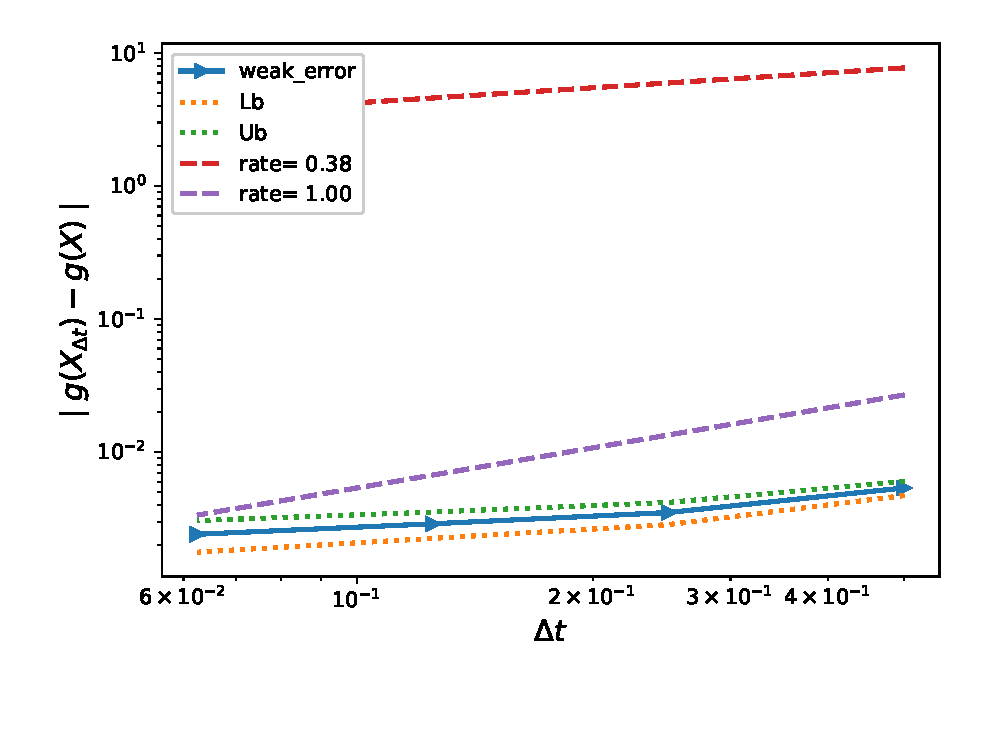
\includegraphics[width=1\linewidth]{./figures/rBergomi_weak_error_rates/without_richardson/H_002/weak_convergence_order_Bergomi_H_002_K_08_M_5_10_6_CI_relative}
%		\caption{}
%		\label{fig:sub3}
%	\end{subfigure}%
%	\begin{subfigure}{.35\textwidth}
%		\centering
%		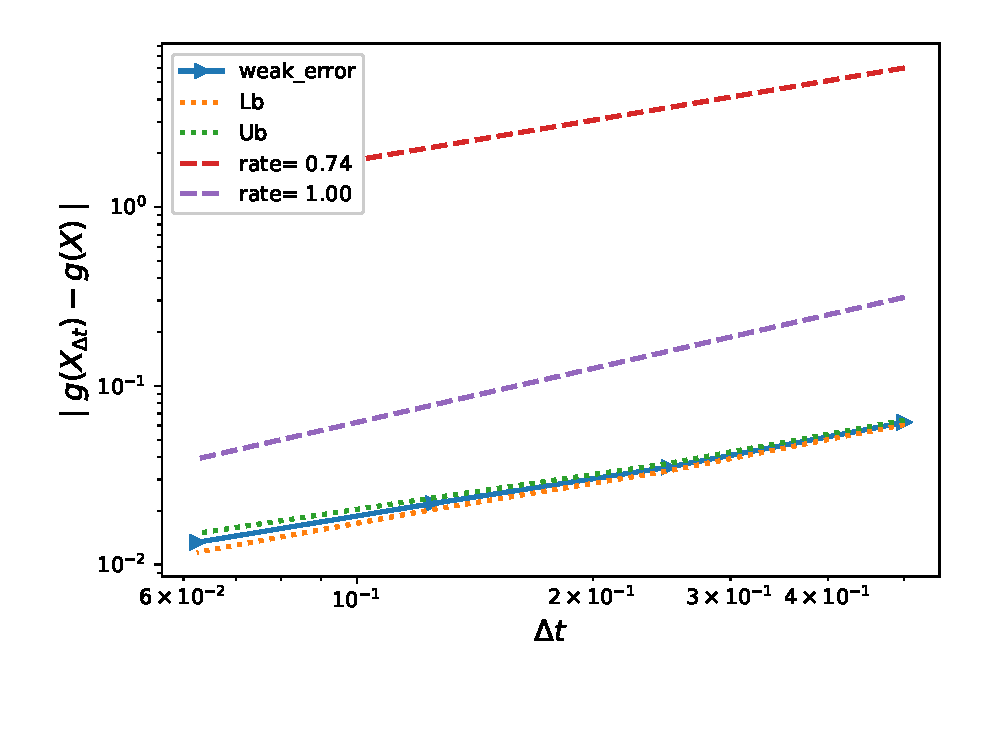
\includegraphics[width=1\linewidth]{./figures/rBergomi_weak_error_rates/without_richardson/H_002/weak_convergence_order_Bergomi_H_002_K_12_M_3_10_6_CI_relative}
%		\caption{}
%		\label{fig:sub4}
%	\end{subfigure}
%	
%	\caption{The rate of convergence of the weak error $\abs{\expt{g(X_{\Delta t})}-g(X)}$  without Richardson extraploation, using MC with $M=5.10^6$: a) Set $3$ parameters in table \ref{table:Reference solution, using MC with $500$ time steps, of Call option price under rBergomi model, for different parameter constellation.},  b) Set $4$ parameters in table \ref{table:Reference solution, using MC with $500$ time steps, of Call option price under rBergomi model, for different parameter constellation.}. }
%	\label{fig:Weak_rate_H_002_without_rich_K_1_K_08}
%\end{figure}

\FloatBarrier









%\begin{figure}[!htb]
%		\centering
%		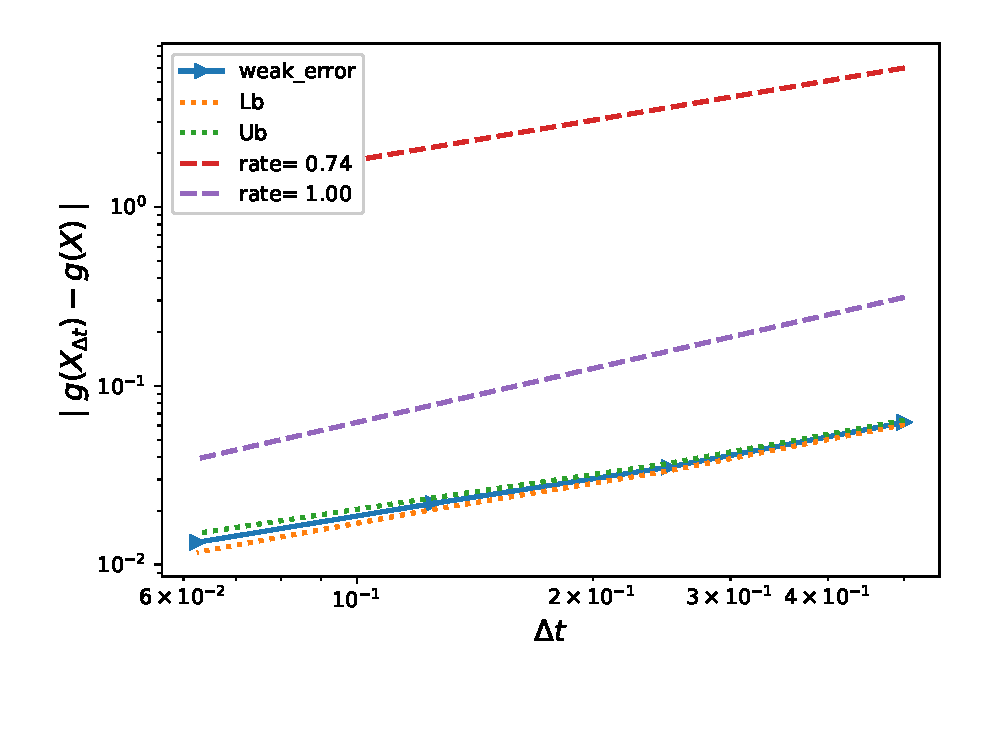
\includegraphics[width=0.35\linewidth]{./figures/rBergomi_weak_error_rates/without_richardson/H_002/weak_convergence_order_Bergomi_H_002_K_12_M_3_10_6_CI_relative}	
%	\caption{The rate of convergence of the weak error $\abs{\expt{g(X_{\Delta t})}-g(X)}$, for set $5$ parameters in table \ref{table:Reference solution, using MC with $500$ time steps, of Call option price under rBergomi model, for different parameter constellation.}, without Richardson extraploation, using MC with $M=5.10^6$.}
%	\label{fig:Weak_rate_H_002_without_rich_K_12}
%\end{figure}




%\subsubsection{With Richardson extrapolation (level 1)}

%\FloatBarrier
%\begin{figure}[h!]
%	\centering
%	\begin{subfigure}{.35\textwidth}
%		\centering
%		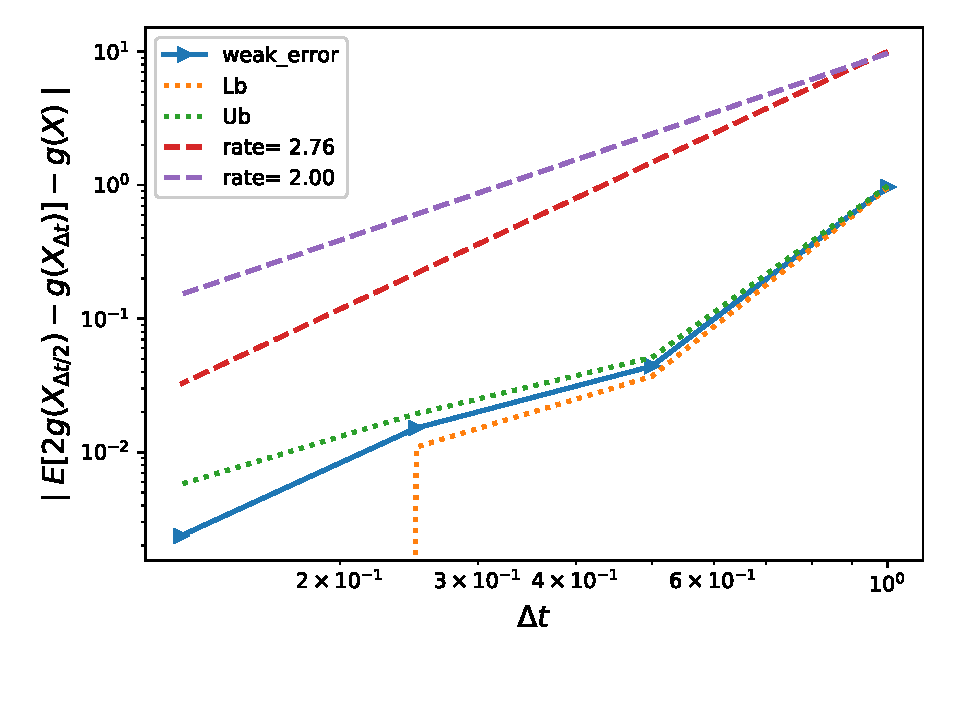
\includegraphics[width=1\linewidth]{./figures/rBergomi_weak_error_rates/with_richardson/H_007/weak_convergence_order_Bergomi_H_007_K_1_richardson_relative_M_10_6}
%		\caption{}
%		\label{fig:sub3}
%	\end{subfigure}%
%	\begin{subfigure}{.35\textwidth}
%		\centering
%		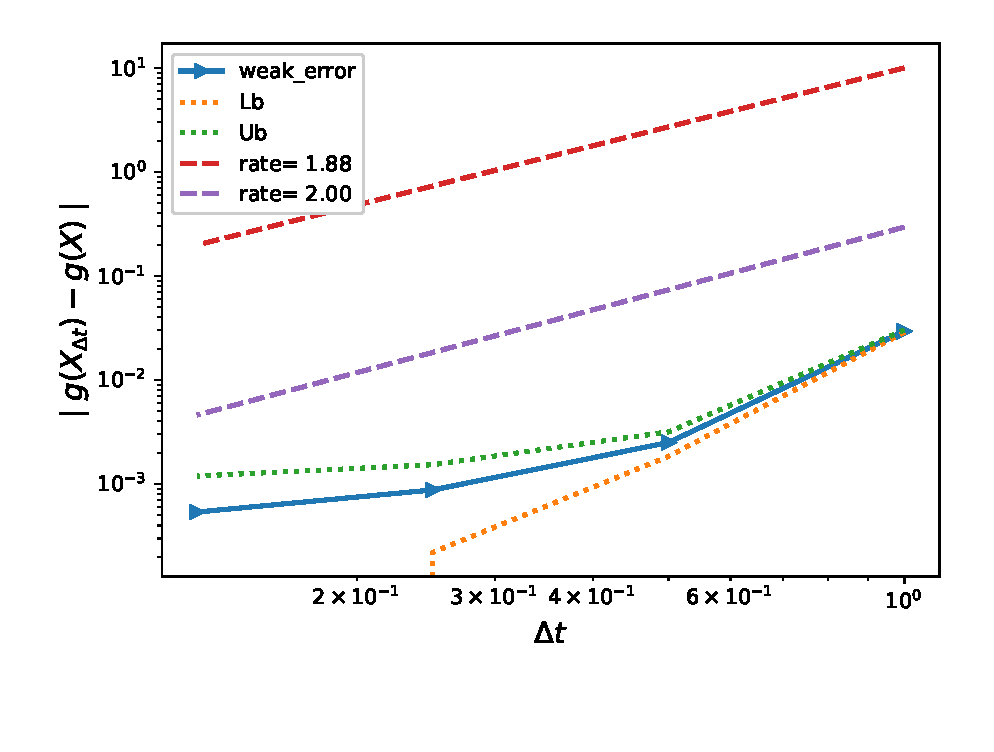
\includegraphics[width=1\linewidth]{./figures/rBergomi_weak_error_rates/with_richardson/H_002/weak_convergence_order_Bergomi_H_002_K_1_M_1_10_7_richardson_relative}
%		\caption{}
%		\label{fig:sub4}
%	\end{subfigure}
%	
%	\caption{The rate of convergence of the weak error  $\abs{\expt{2 g(X_{\Delta t/2}) -g(X_{\Delta t})}-g(X)}$   with Richardson extraploation, using MC with $M=10^6$: a) Set $1$ parameters in table \ref{table:Reference solution, using MC with $500$ time steps, of Call option price under rBergomi model, for different parameter constellation.}.  b) Set $2$ parameters in table \ref{table:Reference solution, using MC with $500$ time steps, of Call option price under rBergomi model, for different parameter constellation.}, }
%	\label{fig:Weak_rate_H_043_007_with_rich}
%\end{figure}
%
%
\FloatBarrier

%\begin{figure}[!htbp]
%	\centering
%		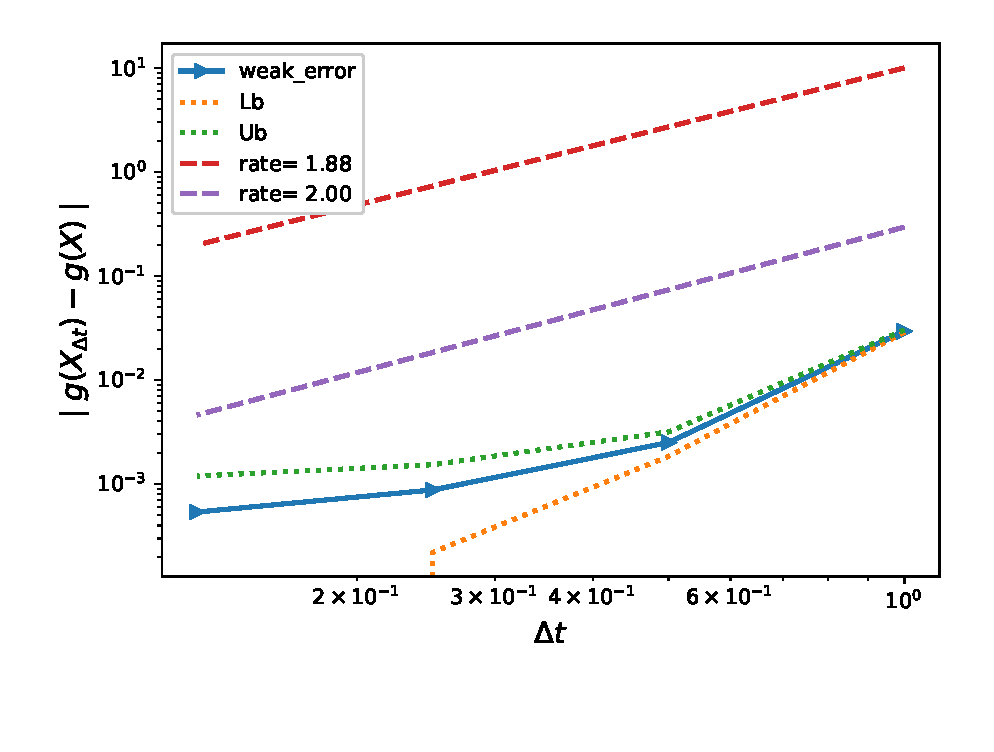
\includegraphics[width=0.35\linewidth]{./figures/rBergomi_weak_error_rates/with_richardson/H_002/weak_convergence_order_Bergomi_H_002_K_1_M_1_10_7_richardson_relative}
%	\caption{The rate of convergence of the weak error $\abs{\expt{2 g(X_{\Delta t/2}) -g(X_{\Delta t})}-g(X)}$,  for set $3$ parameters in table \ref{table:Reference solution, using MC with $500$ time steps, of Call option price under rBergomi model, for different parameter constellation.}, with Richardson extraploation, using MC with $M=10^7$. }
%	\label{fig:Weak_rate_H_002_with_rich_K1}
%\end{figure}
%\FloatBarrier

\subsection{Comparing the errors and computational time for MC, QMC and ASGQ}\label{sec:Comparing different  errors and complexity for MC and MISC}
In this section, we conduct a comparison between MC, QMC and ASGQ in terms of errors and computational time. We show tables and plots reporting  the different relative errors involved in the MC and QMC  methods (bias and statistical error  estimates), and in ASGQ (bias and quadrature error estimates).  While fixing  a  sufficiently small relative error tolerance in the price estimates,  we  compare the computational time needed for all methods to meet the desired error tolerance.  We note that  in all cases the actual work (runtime) is obtained using an Intel(R) Xeon(R) CPU E$5$-$268$ architecture. 

Through our conducted numerical experiments for each parameter set, we follow these steps to achieve our reported results:
\begin{enumerate}
\item[i)] For a fixed number of time steps, $N$, we compute an accurate estimate, using a large number of samples, $M$, of the biased  MC solution, $C_{RB}^{N}$. This step also provides us with an estimate of the bias error, $\mathcal{E}_B(N)$, defined by \eqref{eq:total_error_ASGQ}. 
\item[ii)] The estimated  biased solution,  $C_{RB}^{N}$, is used as a reference solution  to the ASGQ method to compute the quadrature error, $\mathcal{E}_Q(\text{TOL}_{\text{ASGQ}},N)$, defined by \eqref{eq:quadrature error}.
\item[iii)] In order to compare the different methods, the number of samples, $M^{\text{QMC}}$ and $M^{\text{MC}}$, are chosen so that  the statistical errors of randomized QMC, $\mathcal{E}_{S,\text{QMC}}(M^{\text{QMC}})$, and MC, $\mathcal{E}_{S,\text{MC}}(M^{\text{MC}})$, satisfy
\begin{align}\label{optimal_number_samples}
\mathcal{E}_{S,\text{QMC}}(M^{\text{QMC}})=\mathcal{E}_{S,\text{MC}}(M^{\text{MC}})= \mathcal{E}_B(N)=\frac{\mathcal{E}_{\text{tot}}}{2}\COMMA
\end{align}
where $\mathcal{E}_B(N)$ is the bias as defined in \eqref{eq:total_error_ASGQ} and
$\mathcal{E}_{\text{tot}}$ is the total error. 
\end{enumerate}

We show  the summary of our numerical findings in Table \ref{table:Summary of our numerical results.}, which  highlights the computational gains achieved by ASGQ and QMC over \red{the} MC method to meet a certain error tolerance, which we set approximately to $1\%$. We note that the results are reported using the best configuration with Richardson extrapolation for each method. More detailed results for each case of parameter set, as in Table \ref{table:Reference solution, using MC with $500$ time steps, of Call option price under rBergomi model, for different parameter constellation.},  are provided in  Sections \ref{sec:Case of set $2$ parameters_linear}, \ref{sec:Case of set 3 parameters}, \ref{sec:Case of set 4 parameters} and \ref{sec:Case of set 5 parameters}. 
\FloatBarrier
\begin{table}[!h]
	\centering
	\begin{small}
	\begin{tabular}{l*{4}{c}r}
	\toprule[1.5pt]
		Parameter set              &  Total relative error  & CPU time ratio $\left(\text{ASGQ}/\text{MC} \right)$ & CPU time ratio  $\left( \text{QMC}/\text{MC} \right)$\\
		\hline
			Set $1$  &  $1\%$&  $ 6.7\%$ &  $10\%$\\	
           	
              \hline
            Set $2$     &  $0.2\%$&  $4.7\%$ &  $1.4\%$\\		
				 \hline
					Set $3$    &  $0.4\%$&  $3.8\%$ &  $4.7\%$\\	
					\hline
						Set $4$  &  $2\%$&  $20\%$ &  $10\%$\\	
		\bottomrule[1.25pt]
	\end{tabular}
\end{small}
	\caption{Summary of relative errors and computational gains, achieved by the different methods. In this table, we highlight the computational gains achieved by ASGQ and QMC over \red{the} MC method to meet a certain error tolerance. We note that the ratios are computed for the best configuration with Richardson extrapolation for each method. We provide details about the way we compute these gains for each case in the following sections.}
	\label{table:Summary of our numerical results.}
\end{table}
\FloatBarrier

	
	



%\subsubsection{Case of set $1$ parameters in table \ref{table:Reference solution, using MC with $500$ time steps, of Call option price under rBergomi model, for different parameter constellation.}}\label{sec:Case of set 1 parameters}
%
%\subsubsection*{Without Richardson extrapolation}
%%\begin{table}[h!]
%%	\centering
%%	\begin{tabular}{l*{6}{c}r}
%%		Method \textbackslash  Steps            & $2$ & $4$ & $8$ & $16$ &   \\
%%		\hline
%%%		MISC ($\text{TOL}_{\text{MISC}}=5.10^{-1}$)  & $0.1140$ & $0.0961$ & $0.0848$ & $0.0781$  \\
%%		MISC ($\text{TOL}_{\text{MISC}}=10^{-1}$)  & $0.1140$ & $0.0961$ & $0.0871$ & $0.0802$  \\
%%%		MISC ($\text{TOL}_{\text{MISC}}=5.10^{-2}$)  & $0.1140$ & $0.0963$ & $0.0843$ & $0.0824$  \\
%%		MISC ($\text{TOL}_{\text{MISC}}=10^{-2}$)  & $0.1077$ & $0.0944$ & $0.0838$ & $0.0772$  \\
%%
%%		MISC ($\text{TOL}_{\text{MISC}}=10^{-3}$)  & $0.1077$ & $0.0921$ & $0.0819$ & $0.0762$  \\
%%%		MISC ($\text{TOL}_{\text{MISC}}=5.10^{-4}$)  & $0.1079   $ & $0.0921$ & $0.0822$ & $0.0762$  \\
%%		MISC ($\text{TOL}_{\text{MISC}}=10^{-4}$)  & $0.1079$ & $0.0921$ & $0.0822$ & $-$  \\
%%		\hline
%%		MC method ($M=8.10^{6}$)   & $  0.1078$ & $ 0.0921
%%		$  & $   0.0822
%%		$ & $ 0.0767$ \\		
%%		
%%		\hline
%%	\end{tabular}
%%	\caption{ Call option price of the different methods for different number of time steps. Case of set $1$ parameters in table \ref{table:Reference solution, using MC with $500$ time steps, of Call option price under rBergomi model, for different parameter constellation.}, without Richardson extrapolation.}
%%	\label{table: Call option price of the different methods for different number of time steps. Case set 1}
%%\end{table}
%
%
%\begin{table}[h!]
%	\centering
%	\begin{tabular}{l*{6}{c}r}
%		Method \textbackslash  Steps            & $2$ & $4$ & $8$ & $16$  \\
%		\hline
%		MC Bias ($M=8.10^6$)   & 	$ \underset{( 0.0366)}{\mathbf{0.5142}}$  & $\underset{( 0.0209)}{\mathbf{0.2933}}$  & $\underset{( 0.0110)}{\mathbf{0.1551}}$ & $\underset{( 0.0055)}{\mathbf{0.0777}}$\\ 
%		
%		MC Statistical error ($M=8.10^6$)  &  $\underset{(  6.0e-05)} {\mathbf{8.4e-04}}$  & $\underset{(3.4e-05)} {\mathbf{4.8e-04}}$  & $\underset{(2.7e-05)} {\mathbf{ 3.8e-04}}$ & $\underset{( 2.35e-05)} {\mathbf{3.3e-04}}$	\\
%
%		\hline
%	\end{tabular}
%	\caption{Bias and statistical errors of MC  for computing call option price  for different number of time steps. Case set $1$, without Richardson extrapolation. The numbers between parentheses are the corresponding absolute errors.}
%	\label{Bias and Statistical errors of MC ($M=10^6$)  for computing Call option price  for different number of time steps. Case set 1, without Richardson extrapolation. The numbers between parentheses are the corresponding absolute errors.}
%\end{table}
%
%
%
%
%
%
%\FloatBarrier
%
%\begin{figure}[h!]
%	\centering
%	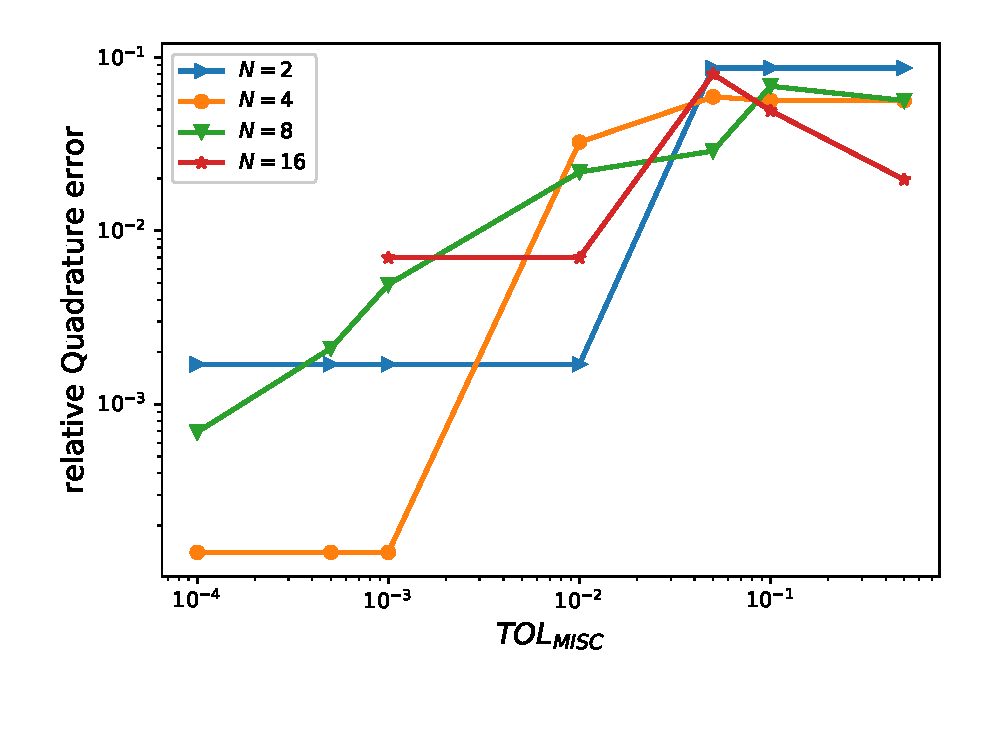
\includegraphics[width=0.35\linewidth]{./figures/rBergomi_MISC_quadratre_error/vs_TOL/set1/relative_quad_error_wrt_MISC_TOL_set1_non_rich}
%	
%	
%	\caption{Quadrature error of MISC, with different tolerances, to compute call option price for different number of time steps. Case  set $1$ parameters, without Richardson extrapolation. See detailed values  in table \ref{Quadrature error of MISC to compute Call option price of the different tolerances for different number of time steps. Case  set $1$ parameters, without Richardson extrapolation. The numbers between parentheses are the corresponding absolute errors.}}
%	\label{fig:Quadrature_error_set1}
%\end{figure}
%
%\FloatBarrier
%
%
%\begin{table}[h!]
%	\centering
%	\begin{tabular}{l*{6}{c}r}
%		Method \textbackslash  Steps            & $2$ & $4$ & $8$ & $16$  \\
%		\hline
%%		MISC ($\text{TOL}_{\text{MISC}}=5.10^{-1}$)  & $\mathbf{0.6010}$ & $\mathbf{0.3496}$ & $\mathbf{ 0.2114}$ & $\mathbf{ 0.0974}$  \\
%		MISC ($\text{TOL}_{\text{MISC}}=10^{-1}$)  & $\mathbf{0.6010}$ & $\mathbf{0.3496}$ & $\mathbf{  0.2232}$ & $\mathbf{
%			0.1269}$  \\
%%		MISC ($\text{TOL}_{\text{MISC}}=5.10^{-2}$)  &$\mathbf{0.6010}$ & $\mathbf{  0.3524}$ & $\mathbf{ 0.1839}$ & $\mathbf{  0.1577}$  \\
%		MISC ($\text{TOL}_{\text{MISC}}=10^{-2}$)  & $\mathbf{\red{0.5159}}$ & $\mathbf{0.3257}$ & $\mathbf{ 0.1769}$ & $\mathbf{  \red{0.0847}}$  \\
%		MISC ($\text{TOL}_{\text{MISC}}=10^{-3}$)  & $\mathbf{0.5159}$ & $\mathbf{\red{0.2934}}$ & $\mathbf{0.1600}$ & $\mathbf{0.0847}$  \\
%%		MISC ($\text{TOL}_{\text{MISC}}=5.10^{-4}$)  & $\mathbf{0.5159}$ & $\mathbf{0.2934}$ & $\mathbf{0.1572}$ & $\mathbf{-}$  \\
%		MISC ($\text{TOL}_{\text{MISC}}=10^{-4}$)  & $\mathbf{0.5159}$ & $\mathbf{0.2934}$ & $\mathbf{\red{0.1558}}$ & $\mathbf{-}$  \\
%		\hline
%		MC     & $\mathbf{\red{0.5159}}$ & $\mathbf{\red{0.2938}}$ & $\mathbf{\red{0.1555}}$ &$\mathbf{  \red{0.0817}}$  \\	
%		
%		\hline
%	\end{tabular}
%	\caption{Total relative error of MISC, with different tolerances,  and MC to compute call option price for different number of time steps. Case  set $1$ parametrs of table \ref{table:Reference solution, using MC with $500$ time steps, of Call option price under rBergomi model, for different parameter constellation.}, without Richardson extrapolation. The values marked in red, for MISC method, correspond to the total relative errors associated with  stable quadrature errors for MISC, and will be used for complexity comparison against MC.}
%	\label{Total error of MISC and MC to compute Call option price of the different tolerances for different number of time steps. Case set 1, without Richardson extrapolation. The numbers between parentheses are the corresponding absolute errors.}
%\end{table}
%
%
%
%\begin{table}[h!]
%	\centering
%	\begin{tabular}{l*{6}{c}r}
%		Method \textbackslash  Steps            & $2$ & $4$ & $8$ & $16$ &   \\
%		\hline
%%		MISC ($\text{TOL}_{\text{MISC}}=5.10^{-1}$)  & $0.1$ & $0.1$ & $0.2$ & $0.4$  \\
%		MISC ($\text{TOL}_{\text{MISC}}=10^{-1}$)  & $0.1$ & $0.1$ & $0.6$ & $6$  \\
%%		MISC ($\text{TOL}_{\text{MISC}}=5.10^{-2}$)  & $0.1$ & $0.3$ & $2$ & $14$  \\
%		MISC ($\text{TOL}_{\text{MISC}}=10^{-2}$)  & $\red{0.2}$ & $1$ & $9$ & $\red{215}$  \\
%		MISC ($\text{TOL}_{\text{MISC}}=10^{-3}$)  & $2$ & $\red{11}$ & $243$ & $4650$  \\
%%		MISC ($\text{TOL}_{\text{MISC}}=5.10^{-4}$)  & $3$ & $17$ & $ 670$ & $-$  \\
%		MISC ($\text{TOL}_{\text{MISC}}=10^{-4}$)  & $6$ & $96$ & $\red{5760}$ & $-$  \\
%		\hline
%		MC     & $\red{ 50}$  & $\red{344}$  & $\red{637}$ & $\red{8}$  \\
%		
%		\hline
%		Ratio of $\left(\text{MC}/ \text{MISC} \right)$  &$\red{  250}$ & $\red{    31
%		}$  & $\red{ 0.1
%		}$  & $\red{  0.04}$ \\
%		\hline
%	\end{tabular}
%	\caption{Comparison of the computational time (in Seconds) of  MC and MISC, used to compute call option price of the rBergomi model for different number of time steps. Case set $1$ parametrs of table \ref{table:Reference solution, using MC with $500$ time steps, of Call option price under rBergomi model, for different parameter constellation.}. The
%		average MC CPU time is computed over 10 runs. }
%	\label{Comparison of the computational time of  MC and MISC, used to compute Call option price of rBergomi model for different number of time steps. Case set1}
%\end{table}
%
%\FloatBarrier
%\subsubsection*{With Richardson extrapolation (level $1$)}
%
%
%
%
%
%
%
%%\begin{table}[h!]
%%	\centering
%%	\begin{tabular}{l*{6}{c}r}
%%		Method \textbackslash  Steps    &$1-2$         & $2-4$ & $4-8$ \\
%%		\hline
%%%		MISC ($\text{TOL}_{\text{MISC}}=5.10^{-1}$)& $0.1357$  & $0.0783$ & $0.0735$ \\
%%		MISC ($\text{TOL}_{\text{MISC}}=10^{-1}$)  &$0.1357$  &$0.0783$ & $0.0785$   \\
%%%		MISC ($\text{TOL}_{\text{MISC}}=5.10^{-2}$)  & $0.1357$ & $0.0831$ & $0.0773$   \\
%%		MISC ($\text{TOL}_{\text{MISC}}=10^{-2}$)  & $0.1237$ &$0.0781$ & $0.0745$   \\
%%
%%		MISC ($\text{TOL}_{\text{MISC}}=10^{-3}$)  & $0.1224$ &$0.0766$ & $0.0720$  \\
%%%		MISC ($\text{TOL}_{\text{MISC}}=10^{-4}$)  &$0.1224$ & $0.0763$ & $0.0724$ \\
%%		\hline
%%		MC method ($M=10^6$)  &$	0.1237$ & $0.0752$ & $0.0721$ \\
%%		\hline
%%	\end{tabular}
%%	\caption{Call option price of the different methods for different number of time steps. Case set $1$ parameters of table \ref{table:Reference solution, using MC with $500$ time steps, of Call option price under rBergomi model, for different parameter constellation.}, using Richardson extrapolation (level $1$).}
%%	\label{table:  Call option price of the different methods for different number of time steps. Case set $1$ parameter, using Richardson extrapolation (level $1$)}
%%\end{table}
%
%
%
%
%\begin{table}[h!]
%	\centering
%	\begin{tabular}{l*{6}{c}r}
%		Method \textbackslash  Steps            & $1-2$ & $2-4$ & $4-8$ & $8-16$  \\
%		\hline
%		MC  Bias ($M=10^6$)    &$\underset{( 0.0525)}{\mathbf{0.7378}}$  & $\underset{(    0.0040)}{\mathbf{0.0561}}$  & $\underset{(0.0009 )}{\mathbf{0.0127}}$  & $\underset{(0.0001)}{\mathbf{0.0021}}$ \\	
%		
%		MC Statistical error ($M=10^6$)   & $\underset{( 2.3e-04)}{\mathbf{3.3e-03}}$  & $\underset{(  1.1e-04)}{\mathbf{1.6e-03}}$  & $\underset{(7.1e-05)}{\mathbf{1.0e-03}}$ & $\underset{(   6.4e-05 )}{\mathbf{9.0e-04}}$ \\	
%		
%		
%		\hline
%	\end{tabular}
%	\caption{Bias and statistical errors of MC   for computing call option price  for different number of time steps. Case set $1$ parameters in tabel \ref{table:Reference solution, using MC with $500$ time steps, of Call option price under rBergomi model, for different parameter constellation.}, with Richardson extrapolation (level $1$). The numbers between parentheses are the corresponding absolute errors.}
%	\label{Bias and Statistical errors of MC ($M=10^6$)  for computing Call option price  for different number of time steps. Case set $1$ parameters, with Richardson extrapolation (level1). The numbers between parentheses are the corresponding absolute errors.}
%\end{table}
%
%
%
%
%
%
%
%
%\begin{figure}[h!]
%	\centering
%	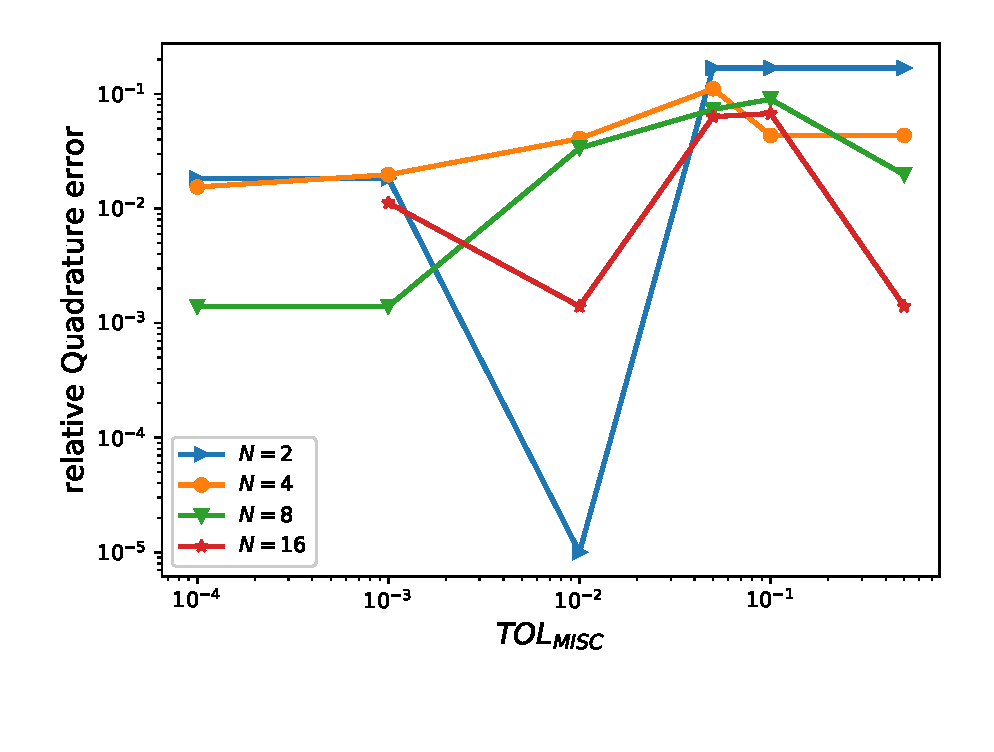
\includegraphics[width=0.35\linewidth]{./figures/rBergomi_MISC_quadratre_error/vs_TOL/set1/relative_quad_error_wrt_MISC_TOL_set1_with_rich}
%	
%	
%	\caption{Quadrature error of MISC, with different tolerances, to compute call option price for different number of time steps. Case  set $1$ parameters, with Richardson extrapolation.  See detailed values  in table \ref{Quadrature error of MISC to compute Call option price of the different tolerances for different number of time steps. Case set $1$ parameters, with Richardson extrapolation(level $1$). The numbers between parentheses are the corresponding absolute errors.}.}
%\end{figure}
%
%
%
%\begin{table}[!h]
%	\centering
%	\begin{tabular}{l*{6}{c}r}
%		Method \textbackslash  Steps            & $1-2$ & $2-4$ & $4-8$   \\
%		\hline
%%		MISC ($\text{TOL}_{\text{MISC}}=5.10^{-1}$)  & $\mathbf{0.9063
%%		}$ & $\mathbf{ 0.0996}$ & $\mathbf{0.0324
%%		}$  \\
%		MISC ($\text{TOL}_{\text{MISC}}=10^{-1}$)  & $\mathbf{0.9063
%		}$ & $\mathbf{ 0.0996}$ & $\mathbf{  0.1026}$   \\
%%		MISC ($\text{TOL}_{\text{MISC}}=5.10^{-2}$)  & $\mathbf{0.9063
%%		}$ & $\mathbf{    0.1670}$ & $\mathbf{ 0.0857}$  \\
%		MISC ($\text{TOL}_{\text{MISC}}=10^{-2}$)  & $\mathbf{0.7378}$ & $\mathbf{  0.0968}$ & $\mathbf{   0.0464}$  \\	
%		MISC ($\text{TOL}_{\text{MISC}}=10^{-3}$)  & $\mathbf{\red{0.7561}}$ & $\mathbf{\red{0.0758}}$ & $\mathbf{\red{0.0141}}$  \\
%%		MISC ($\text{TOL}_{\text{MISC}}=10^{-4}$)  & $\mathbf{0.7561}$ & $\mathbf{0.0715}$ & $\mathbf{0.0141}$ \\
%		\hline
%		MC   & $\mathbf{\red{0.7561}}$  & $\mathbf{\red{0.0758}}$  & $\mathbf{\red{0.0141}}$  \\
%		
%		\hline
%	\end{tabular}
%	\caption{Total  relative error of MISC and MC, with different tolerances, to compute call option price for different number of time steps. Case set $1$ parameters in table \ref{table:Reference solution, using MC with $500$ time steps, of Call option price under rBergomi model, for different parameter constellation.}, with Richardson extrapolation(level $1$). The values marked in red, for MISC method, correspond to the total relative errors associated with  stable quadrature errors for MISC, and will be used for complexity comparison against MC.}
%	\label{Total  error of MISC and MC to compute Call option price of the different tolerances for different number of time steps. Case set $1$ parameters, with Richardson extrapolation(level $1$). The numbers between parentheses are the corresponding absolute errors.}
%\end{table}
%\FloatBarrier
%\begin{table}[!h]
%	\centering
%	\begin{tabular}{l*{6}{c}r}
%		Method \textbackslash  Steps            & $1-2$ & $2-4$ & $4-8$   \\
%		\hline
%%		MISC ($\text{TOL}_{\text{MISC}}=5.10^{-1}$)  & $0.1$ & $0.1$ & $0.2$  \\
%		MISC ($\text{TOL}_{\text{MISC}}=10^{-1}$)  & $0.1$ & $0.1$ & $0.6$ \\
%%		MISC ($\text{TOL}_{\text{MISC}}=5.10^{-2}$)  & $0.1$ & $0.4$ & $2$   \\
%		MISC ($\text{TOL}_{\text{MISC}}=10^{-2}$)  & $1$ & $2$ & $18$   \\
%		MISC ($\text{TOL}_{\text{MISC}}=10^{-3}$)  & $\red{4}$ & $\red{12}$ & $\red{520}$   \\	
%%		MISC ($\text{TOL}_{\text{MISC}}=10^{-4}$)  & $7$ & $191$ & $7650$  \\
%		\hline
%		MC   & $\red{ 34.7}$  & $\red{37}$  & $ \red{532}$    \\
%		
%		\hline
%		Ratio of $\left(\text{MC}/ \text{MISC} \right)$  &$\red{8.7}$ & $\red{   3.1
%		}$  & $\red{1}$ \\
%		\hline
%	\end{tabular}
%	\caption{Comparison of the computational time (in Seconds) of  MC and MISC, using Richardson extrapolation (level $1$), used to compute call option price of the rBergomi model for different number of time steps. Case set $1$ parameters in table \ref{table:Reference solution, using MC with $500$ time steps, of Call option price under rBergomi model, for different parameter constellation.}. The
%		average MC CPU time is computed over 10 runs.}
%	\label{Comparsion of the computational time of  MC and MISC, using Richardson extrapolation (level $1$), used to compute Call option price of rBergomi model for different number of time steps. Case set $1$ parameters}
%\end{table}
%
%
%
%
%\FloatBarrier
%
%\subsubsection*{With Richardson extrapolation (level $2$)}
%%\FloatBarrier
%%\begin{table}[h!]
%%	\centering
%%	\begin{tabular}{l*{6}{c}r}
%%		Method \textbackslash  Steps           &$1-2-4$ & $2-4-8$ \\
%%		\hline
%%%		MISC ($\text{TOL}_{\text{MISC}}=5.10^{-1}$)& $0.0591$  & $0.0719$ \\
%%		
%%		MISC ($\text{TOL}_{\text{MISC}}=10^{-1}$)  &$0.0567$  &$0.0747$   \\
%%%		MISC ($\text{TOL}_{\text{MISC}}=5.10^{-2}$)  & $0.0733$ & $0.0782$  \\
%%		MISC ($\text{TOL}_{\text{MISC}}=10^{-2}$)  & $		0.0639$ & $0.0729$   \\
%%		MISC ($\text{TOL}_{\text{MISC}}=5.10^{-3}$)  & $	0.0620$ & $0.0708$   \\
%%%		MISC ($\text{TOL}_{\text{MISC}}=10^{-3}$)  & $	0.0608$ & $0.0708$  \\
%%%		MISC ($\text{TOL}_{\text{MISC}}=10^{-4}$)  & $	0.0608$ & $-$   \\
%%		\hline
%%		MC ($M=3.10^6$)  & $0.0608$ & $0.0710$   \\
%%		\hline 
%%	\end{tabular}
%%	\caption{ Call option price of the different methods for different number of time steps.  Case set $1$ parameters in table \ref{table:Reference solution, using MC with $500$ time steps, of Call option price under rBergomi model, for different parameter constellation.}, using Richardson extrapolation (level $2$).}
%%	\label{table: Call option price of the different methods for different number of time steps. Case $K=1$, using Richardson extrapolation_level2}
%%\end{table}
%
%\FloatBarrier
%
%
%\begin{table}[h!]
%	\centering
%	\begin{tabular}{l*{6}{c}r}
%		Method \textbackslash  Steps            & $1-2-4$ & $2-4-8$  \\
%		\hline
%		MC  Bias ($M=3.10^6$)     &$\underset{( 0.0104)}{\mathbf{ 0.1459}}$  & $\underset{(    1.7e-04)}{\mathbf{0.0024}}$   \\	
%		
%		MC Statistical error ($M=3.10^6$)   & $\underset{( 1.0e-04)}{\mathbf{1.5e-03}}$  & $\underset{(   4.8e-05)}{\mathbf{    6.8e-04}}$  \\	
%		
%		
%		
%		\hline
%	\end{tabular}
%	\caption{Bias and statistical errors of MC   for computing call option price  for different number of time steps. Case set $1$ parameters in tabel \ref{table:Reference solution, using MC with $500$ time steps, of Call option price under rBergomi model, for different parameter constellation.}, with Richardson extrapolation (level $2$). The numbers between parentheses are the corresponding absolute errors.}
%	\label{Bias and Statistical errors of MC ($M=3.10^6$)  for computing Call option price  for different number of time steps. Case set $1$ parameters, with Richardson extrapolation (level2). The numbers between parentheses are the corresponding absolute errors.}
%\end{table}
%
%
%
%
%\FloatBarrier
%\begin{figure}[h!]
%	\centering
%	evel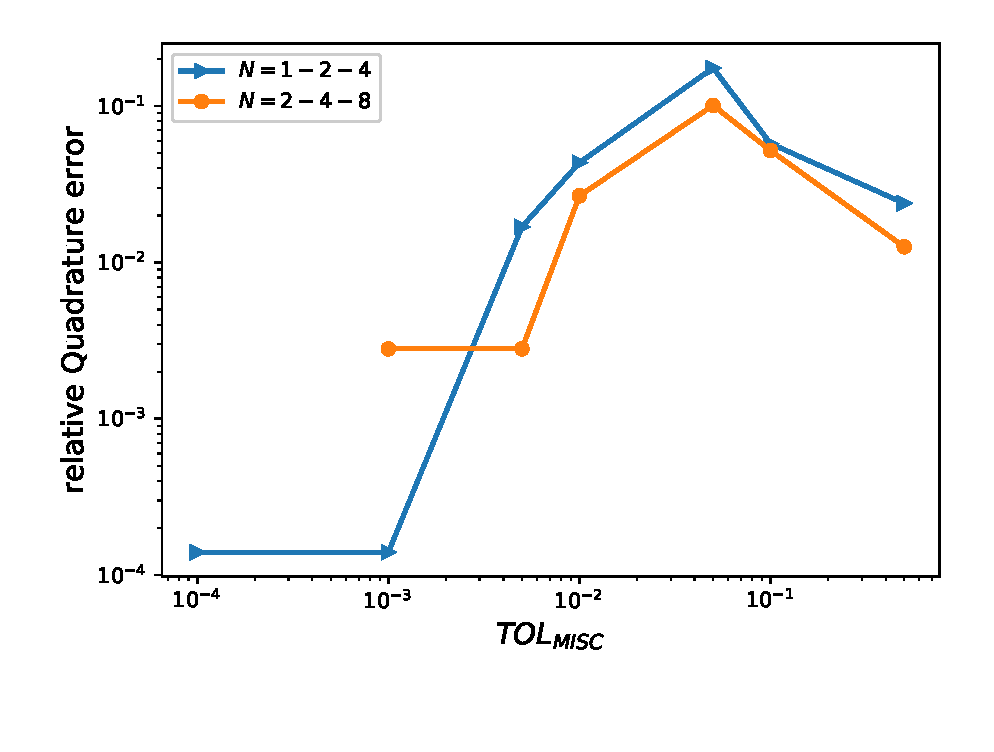
\includegraphics[width=0.35\linewidth]{./figures/rBergomi_MISC_quadratre_error/vs_TOL/set1/relative_quad_error_wrt_MISC_TOL_set1_rich_level2}
%	
%	
%	\caption{Quadrature error of MISC, with different tolerances, to compute call option price of the different tolerances for different number of time steps. Case  set $1$ parameters, with Richardson extrapolation (level $2$).  See detailed values  in table \ref{Quadrature error of MISC to compute Call option price of the different tolerances for different number of time steps. Case set $1$ parameters, with Richardson extrapolation(level $2$). The numbers between parentheses are the corresponding absolute errors.}.}
%	\label{fig:Quadrature_error_set1_rich_level2}
%\end{figure}
%
%
%
%\FloatBarrier
%\begin{table}[!h]
%	\centering
%	\begin{tabular}{l*{6}{c}r}
%		Method \textbackslash  Steps            & $1-2-4$ & $2-4-8$  \\
%		\hline
%%		MISC ($\text{TOL}_{\text{MISC}}=5.10^{-1}$)  & $\mathbf{0.1698
%%		}$ & $\mathbf{ 0.0150}$  \\
%		MISC ($\text{TOL}_{\text{MISC}}=10^{-1}$)  & $\mathbf{0.2035
%		}$ & $\mathbf{ 0.0544}$ \\
%%		MISC ($\text{TOL}_{\text{MISC}}=5.10^{-2}$)  & $\mathbf{0.3214
%%		}$ & $\mathbf{    0.1035}$  \\
%		MISC ($\text{TOL}_{\text{MISC}}=10^{-2}$)  & $\mathbf{0.1894}$ & $\mathbf{  0.0291}$   \\	
%		MISC ($\text{TOL}_{\text{MISC}}=5.10^{-3}$)  & $\mathbf{\red{0.1628}}$ & $\mathbf{\red{0.0052}}$   \\
%%		MISC ($\text{TOL}_{\text{MISC}}=10^{-3}$)  & $\mathbf{0.1460}$ & $\mathbf{0.0052}$   \\
%%		MISC ($\text{TOL}_{\text{MISC}}=10^{-4}$)  & $\mathbf{0.1460}$ & $\mathbf{-}$  \\
%		\hline
%		MC   & $\mathbf{\red{0.1628}}$  & $\mathbf{\red{0.0052}}$    \\
%		\hline
%	\end{tabular}
%	\caption{Total  relative error of MISC, with different tolerances, and MC to compute call option price for different number of time steps. Case set $1$ parameters in table \ref{table:Reference solution, using MC with $500$ time steps, of Call option price under rBergomi model, for different parameter constellation.}, with Richardson extrapolation(level $2$). The values marked in red, for MISC method, correspond to the total relative errors associated with  stable quadrature errors for MISC, and will be used for complexity comparison against MC.}
%	\label{Total  error of MISC and MC to compute Call option price of the different tolerances for different number of time steps. Case set $1$ parameters, with Richardson extrapolation(level $2$). The numbers between parentheses are the corresponding absolute errors.}
%\end{table}
%
%\FloatBarrier
%
%\begin{table}[!h]
%	\centering
%	\begin{tabular}{l*{6}{c}r}
%		Method \textbackslash  Steps            & $1-2-4$ & $2-4-8$   \\
%		\hline
%%		MISC ($\text{TOL}_{\text{MISC}}=5.10^{-1}$)  & $0.2$ & $0.3$  \\
%		MISC ($\text{TOL}_{\text{MISC}}=10^{-1}$)  & $0.25$ & $2$ &   \\
%%		MISC ($\text{TOL}_{\text{MISC}}=5.10^{-2}$)  & $0.55$ & $5$  \\
%		MISC ($\text{TOL}_{\text{MISC}}=10^{-2}$)  & $2$ & $24$   \\
%		MISC ($\text{TOL}_{\text{MISC}}=5.10^{-3}$)  & $\red{5}$ & $\red{64}$  \\	
%%		MISC ($\text{TOL}_{\text{MISC}}=10^{-3}$)  & $24$ & $1067$  \\	
%%		MISC ($\text{TOL}_{\text{MISC}}=10^{-4}$)  & $ 233$ & $-$   \\
%		\hline
%		MC    & $\red{20}$  & $\red{231}$  \\
%		
%		\hline
%		Ratio of $\left(\text{MC}/ \text{MISC} \right)$  &$\red{4}$ & $\red{  3.6}$   \\
%		\hline
%	\end{tabular}
%	\caption{Comparison of the computational time (in Seconds) of  MC and MISC, using Richardson extrapolation (level $2$), used to compute call option price of the rBergomi model for different number of time steps. Case set $1$ parameters in table \ref{table:Reference solution, using MC with $500$ time steps, of Call option price under rBergomi model, for different parameter constellation.}. The
%		average MC CPU time is computed over 10 runs.}
%	\label{Comparsion of the computational time of  MC and MISC, using Richardson extrapolation (level $2$), used to compute Call option price of rBergomi model for different number of time steps. Case set $1$ parameters}
%\end{table}
%
%
%
%\FloatBarrier
%
%
%
%
%
%
%
%\begin{figure}[h!]
%	\centering
%	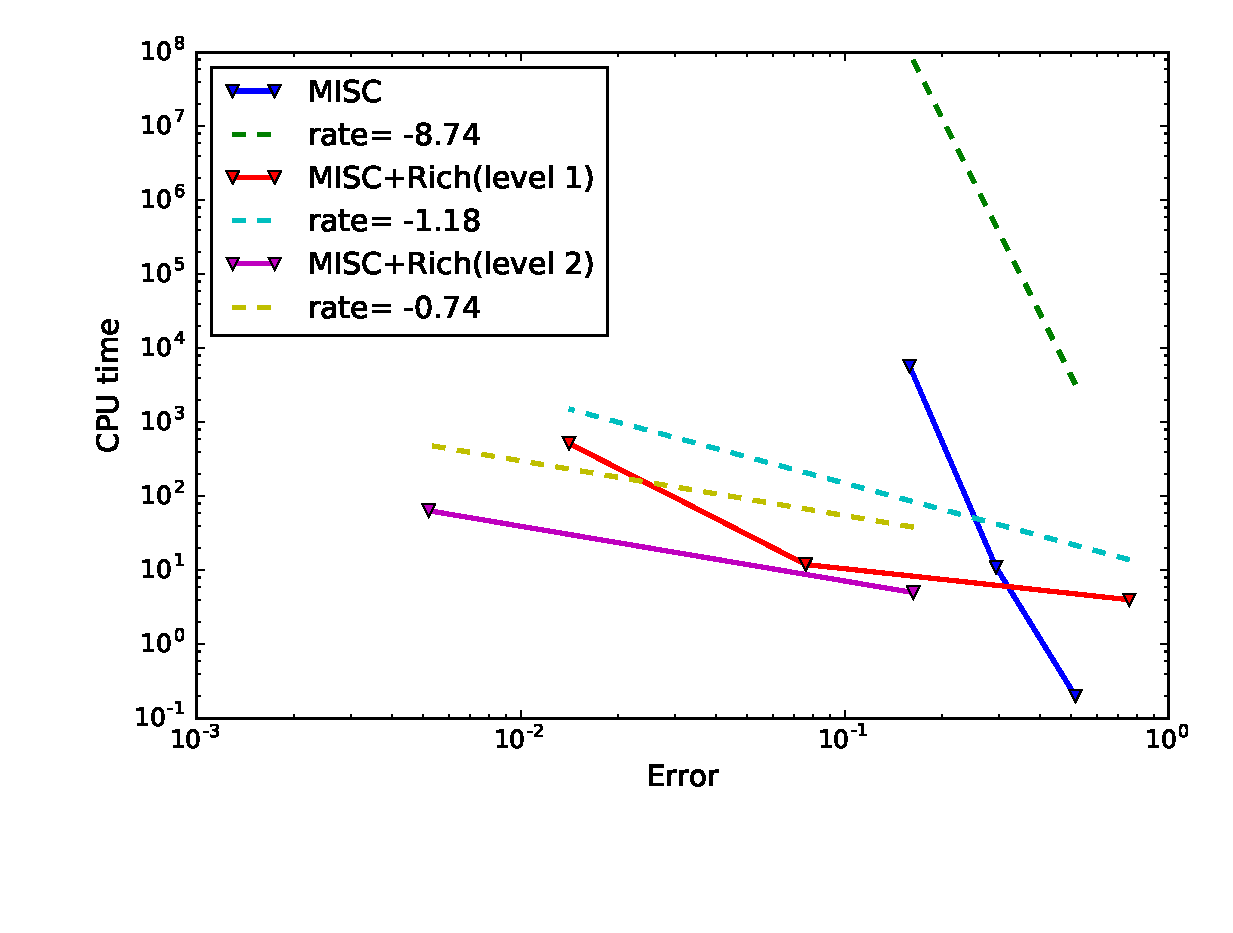
\includegraphics[width=0.35\linewidth]{./figures/rBergomi_Complexity_rates/set1/error_vs_time_set1_comparison}
%	
%	\caption{Complexity plot for  MISC (with and without) Richardson extrapolation for case set $1$ parameters of table \ref{table:Reference solution, using MC with $500$ time steps, of Call option price under rBergomi model, for different parameter constellation.}.}
%	\label{fig:Complexity plot for  MISC for Case set $1$ parameters, comparison}
%\end{figure}
%
%\FloatBarrier
%
%
%


\subsubsection{Case of parameters in Set 1 in Table \ref{table:Reference solution, using MC with $500$ time steps, of Call option price under rBergomi model, for different parameter constellation.} }
\label{sec:Case of set $2$ parameters_linear}
In this section, we conduct our numerical experiments for three different scenarios: i) without Richardson extrapolation, ii) with (level $1$) Richardson extrapolation, and iii) with (level $2$) Richardson extrapolation. Figure \ref{fig: Comparing the numerical complexity of the different  methods with the different configurations}  shows a comparison of the numerical complexity for each method under the three different scenarios. From this Figure, we conclude that to achieve a relative error of $1\%$, level $1$ of Richardson extrapolation is the optimal configuration for both \red{the} MC and \red{the} randomized QMC methods, and level $2$ of Richardson extrapolation is the optimal configuration for \red{the} ASGQ  method.

\FloatBarrier
\begin{figure}[htb]
	\centering % <-- added
	\begin{subfigure}{0.33\textwidth}
		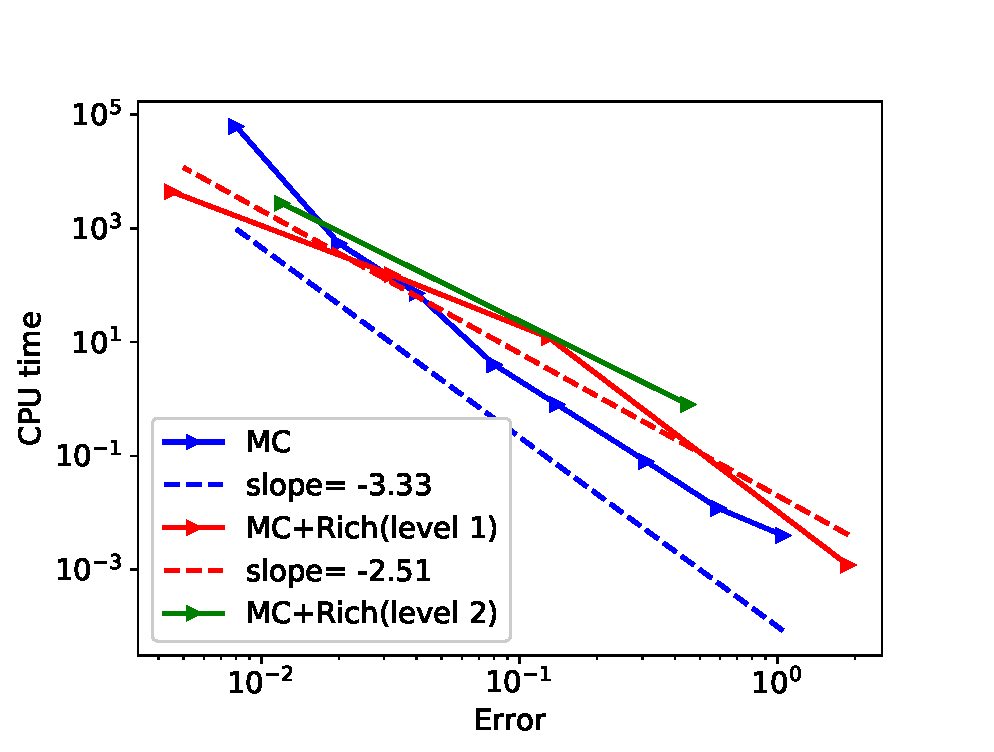
\includegraphics[width=\linewidth]{./figures/rBergomi_Complexity_rates/set2/error_vs_time_set2_MC_comparison}
		\caption{}
		\label{fig:1}
	\end{subfigure}\hfil % <-- added
	\begin{subfigure}{0.33\textwidth}
		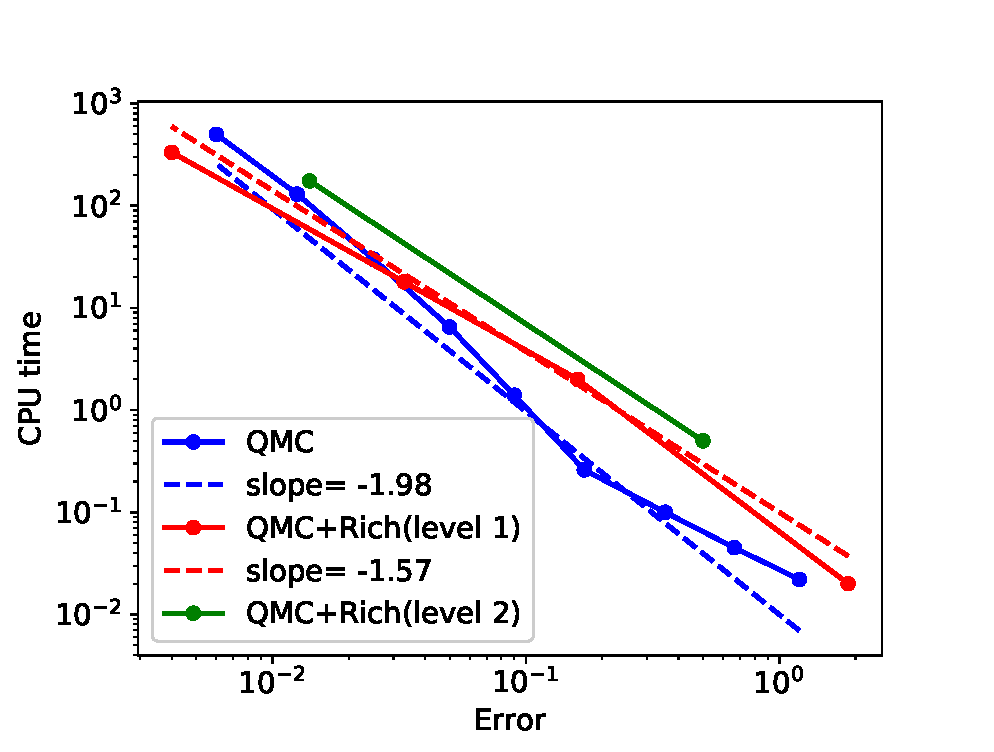
\includegraphics[width=\linewidth]{./figures/rBergomi_Complexity_rates/set2/error_vs_time_set2_QMC_comparison}
		\caption{}
		\label{fig:2}
	\end{subfigure}\hfil % <-- added
	\begin{subfigure}{0.33\textwidth}
		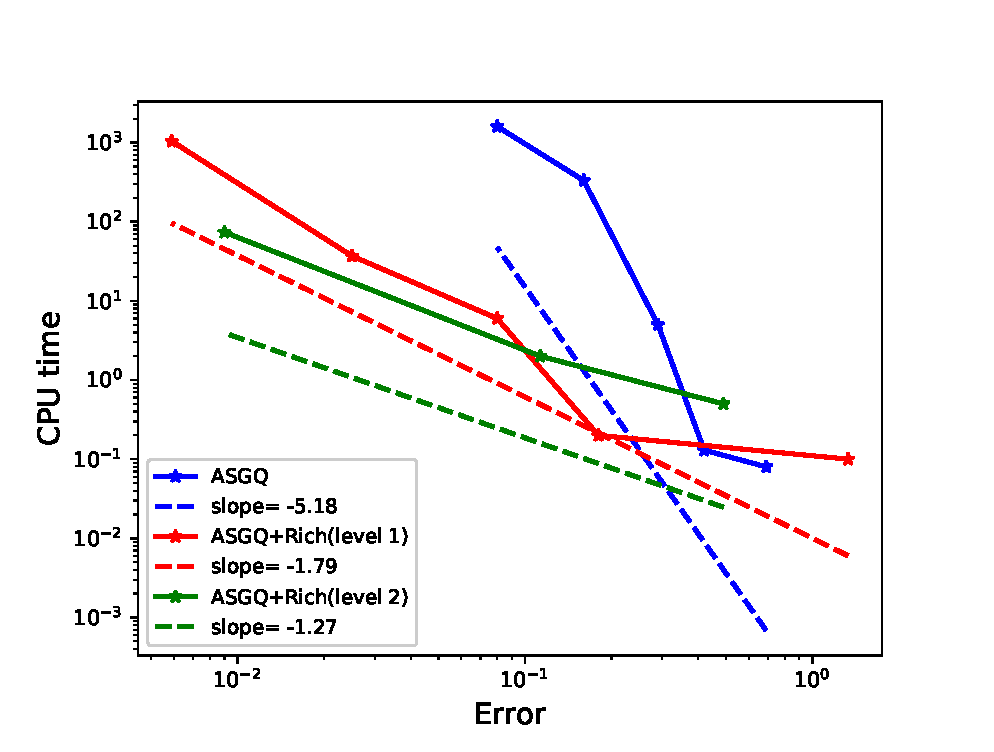
\includegraphics[width=\linewidth]{./figures/rBergomi_Complexity_rates/set2/error_vs_time_set2_MISC_comparison}
		\caption{}
		\label{fig:3}
	\end{subfigure}
	\caption{Comparing the numerical complexity of the different  methods with the different configurations in terms of the level of Richardson extrapolation. a) MC methods. b) QMC methods. d) ASGQ methods.}
	\label{fig: Comparing the numerical complexity of the different  methods with the different configurations}
\end{figure}
\FloatBarrier

We compare these optimal configurations for each method  in Figure \ref{fig:Complexity plot for  MISC for Case set $2$ parameters, comparison}, and we \red{show} that both ASGQ and QMC \red{outperform} MC, in terms of numerical complexity. In particular, to achieve a total relative error \red{of} $1\%$, ASGQ coupled with level $2$ of Richardson extrapolation requires
approximately $6.7\%$ of the work of MC coupled with level $1$ of Richardson extrapolation, and  QMC coupled with level $1$ of Richardson extrapolation requires approximately $10\%$ of the work of MC coupled with level $1$ of Richardson extrapolation. We show more detailed outputs for the methods compared in Figure \ref{fig:Complexity plot for  MISC for Case set $2$ parameters, comparison} in Appendix \ref{appendix:Case of set 1 parameters}.
\FloatBarrier
\begin{figure}[h!]
	\centering
	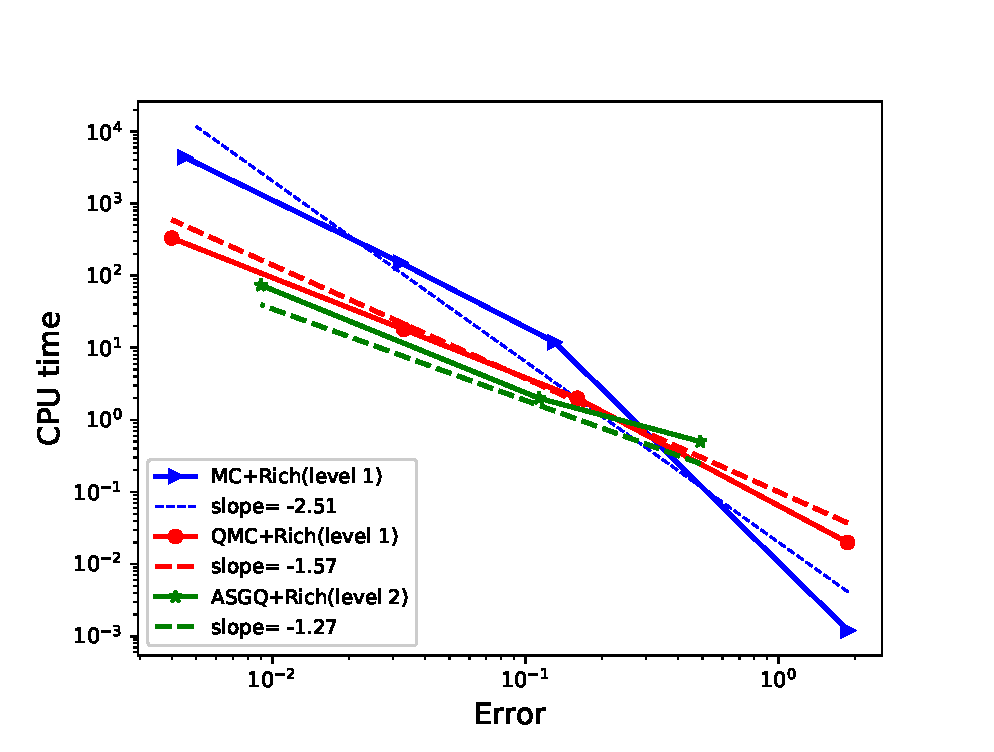
\includegraphics[width=0.4\linewidth]{./figures/rBergomi_Complexity_rates/set2/error_vs_time_set2_full_comparison}
	
	\caption{Computational work comparison for the different methods with the best configurations\red{, as} concluded from Figure \ref{fig: Comparing the numerical complexity of the different  methods with the different configurations}, for the case of parameter set $1$ in Table \ref{table:Reference solution, using MC with $500$ time steps, of Call option price under rBergomi model, for different parameter constellation.}. This plot shows that to achieve a relative error below $1\%$, ASGQ coupled with level $2$ of Richardson extrapolation and QMC coupled with level $1$ of  Richardson extrapolation have the same performance. Furthermore, they outperform significantly \red{the} MC method coupled with level $1$ of Richardson extrapolation.}
	\label{fig:Complexity plot for  MISC for Case set $2$ parameters, comparison}
\end{figure}
\FloatBarrier



\subsubsection{Case of parameters in Set 2  in Table \ref{table:Reference solution, using MC with $500$ time steps, of Call option price under rBergomi model, for different parameter constellation.} }\label{sec:Case of set 3 parameters}

In this section, we only conduct our numerical experiments for the case without Richardson extrapolation, since the results show that we meet a small enough relative error tolerance without the need to apply Richardson extrapolation. We compare the different methods  in Figure \ref{fig:Complexity plot for  MISC for case set $3$ parameters, comparison}, and we \red{determine} that both ASGQ and QMC \red{outperform} MC, in terms of numerical complexity. In particular,  to achieve a total relative error of about $0.2\%$, ASGQ  requires
	approximately $4.7\%$ of the work of MC, and  QMC requires approximately $1.4\%$ of the work of MC. We show more detailed outputs for the methods compared in Figure \ref{fig:Complexity plot for  MISC for case set $3$ parameters, comparison} in Appendix \ref{appendix:Case of set $2$ parameters}. 
\FloatBarrier
	\begin{figure}[h!]
	\centering
	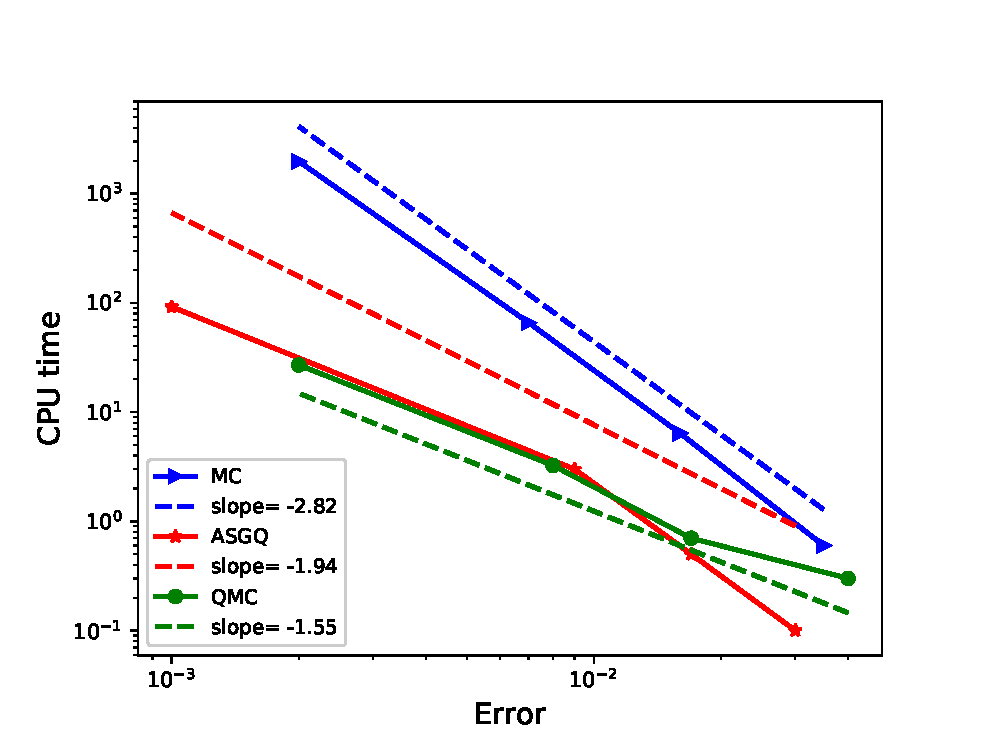
\includegraphics[width=0.4\linewidth]{./figures/rBergomi_Complexity_rates/set5/error_vs_time_set5_full_comparison}
	
	\caption{Computational work comparison for   the different  methods, for the case of parameter set $2$ in Table \ref{table:Reference solution, using MC with $500$ time steps, of Call option price under rBergomi model, for different parameter constellation.}. This plot shows that to achieve a relative error below $1\%$, ASGQ and QMC have similar performance and they outperform  \red{the MC method significantly} in terms of computational time.}
	\label{fig:Complexity plot for  MISC for case set $3$ parameters, comparison}
\end{figure}
\FloatBarrier
\subsubsection{Case of parameters in Set 3  in Table \ref{table:Reference solution, using MC with $500$ time steps, of Call option price under rBergomi model, for different parameter constellation.} }\label{sec:Case of set 4 parameters}
In this section, we only conduct our numerical experiments for the case without Richardson extrapolation, since the results show that we meet a small enough relative error tolerance without the need to apply Richardson extrapolation. We compare the different methods  in Figure \ref{fig:Complexity plot for MC and MISC for case set $4$ parameters}, and we \red{determine} that both ASGQ and QMC \red{outperform} MC, in terms of numerical complexity. In particular,  to achieve a total relative error of about $0.4\%$, ASGQ  requires
	approximately $3.8\%$ of the work of MC, and  QMC requires approximately $4.7\%$ of the work of MC. We show more detailed outputs for the methods compared in Figure \ref{fig:Complexity plot for MC and MISC for case set $4$ parameters} in Appendix \ref{appendix:Case of set 3 parameters}.

\FloatBarrier

\begin{figure}[h!]
	\centering
	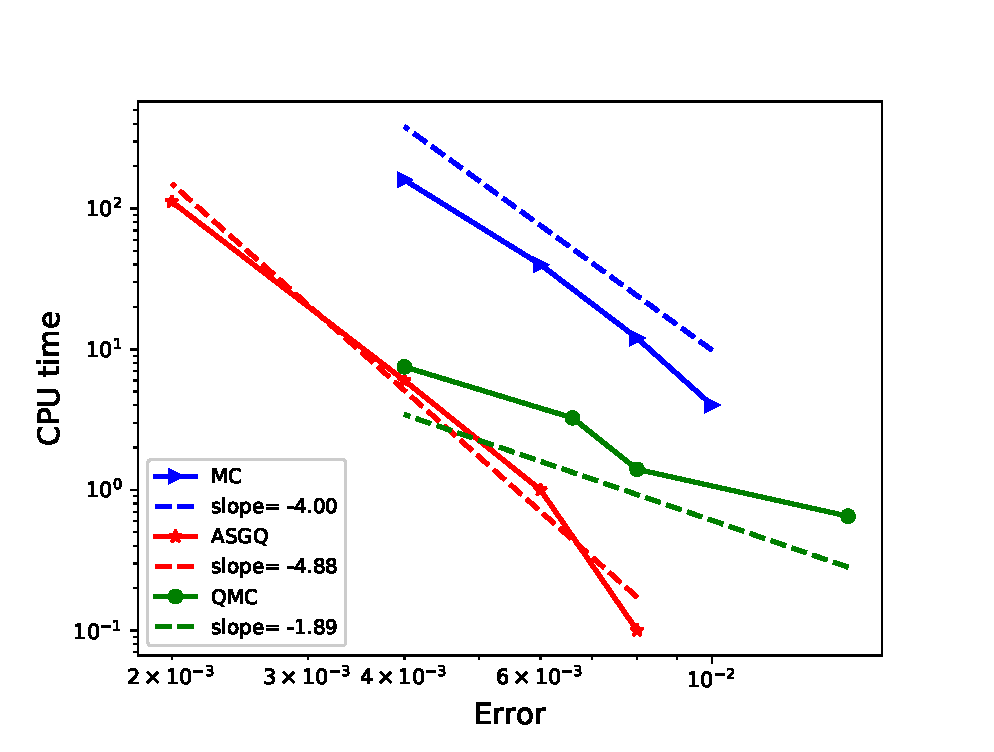
\includegraphics[width=0.4\linewidth]{./figures/rBergomi_Complexity_rates/set6/error_vs_time_set6_full_comparison}
	
	\caption{Comparison of computational work for the different  methods, for the case of parameter set $3$ in Table \ref{table:Reference solution, using MC with $500$ time steps, of Call option price under rBergomi model, for different parameter constellation.}.}
	\label{fig:Complexity plot for MC and MISC for case set $4$ parameters}
\end{figure}
\FloatBarrier

\subsubsection{Case of parameters in Set 4  in Table \ref{table:Reference solution, using MC with $500$ time steps, of Call option price under rBergomi model, for different parameter constellation.} }\label{sec:Case of set 5 parameters}

In this section, we only conduct our numerical experiments for the case without Richardson extrapolation.  We compare the different methods  in Figure \ref{fig:Complexity plot for MC and MISC for Case set $5$ parameters}, and we \red{determine} that both ASGQ and QMC \red{outperform} MC, in terms of numerical complexity. In particular,  to achieve a total relative error of about $2\%$, ASGQ  requires	approximately $20\%$ of the work of MC, and  QMC requires approximately $10\%$ of the work of MC. We show more detailed outputs for the methods compared in Figure \ref{fig:Complexity plot for MC and MISC for Case set $5$ parameters} in Appendix \ref{appendix:Case of set 4 parameters}.   Similar to the case of set $1$ parameters, illustrated in section \ref{sec:Case of set $2$ parameters_linear}, we believe that Richardson extrapolation will improve the performance of \red{the} ASGQ and QMC methods.   We should also point out that, since we are in the out of the money regime in this case, a fairer comparison of the methods may be done after coupling them with an importance sampling method, so that more points are sampled in the right region of the payoff function.
\FloatBarrier
	\begin{figure}[h!]
	\centering
	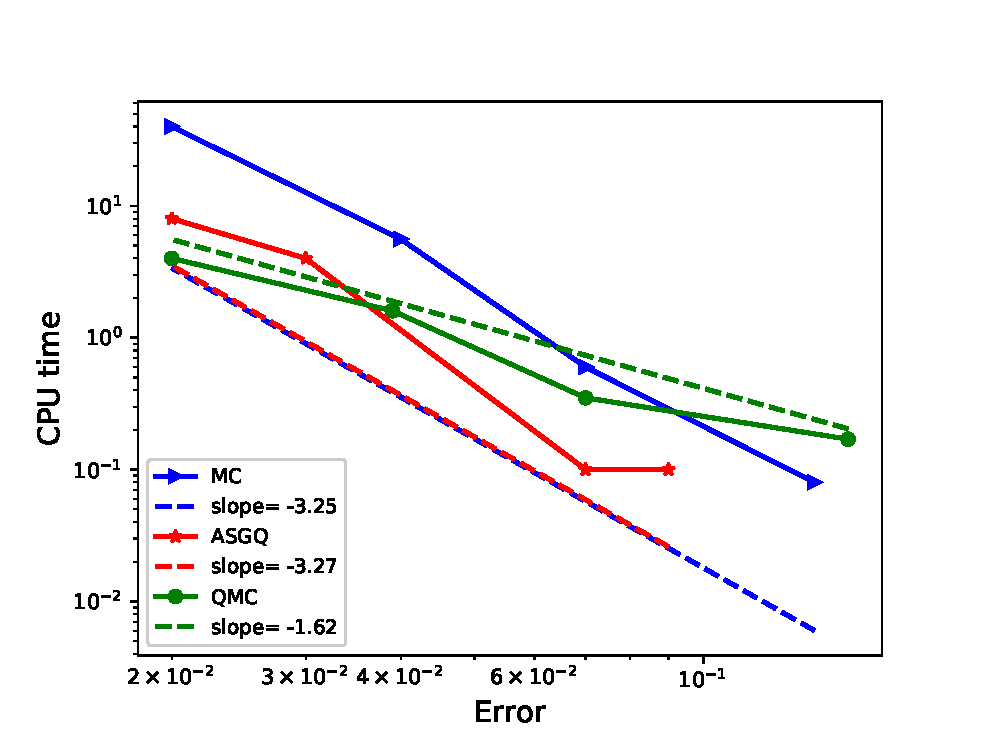
\includegraphics[width=0.4\linewidth]{./figures/rBergomi_Complexity_rates/set7/error_vs_time_set7_full_comparison}
	
	\caption{Comparison of computational work for the different methods, for the case of parameter set $4$ in Table \ref{table:Reference solution, using MC with $500$ time steps, of Call option price under rBergomi model, for different parameter constellation.}.}
	\label{fig:Complexity plot for MC and MISC for Case set $5$ parameters}
\end{figure}
\FloatBarrier






